\documentclass[tikz,border=10pt]{standalone}
\usepackage{tikz}
\usetikzlibrary{arrows.meta, positioning, decorations.pathmorphing}

\begin{document}
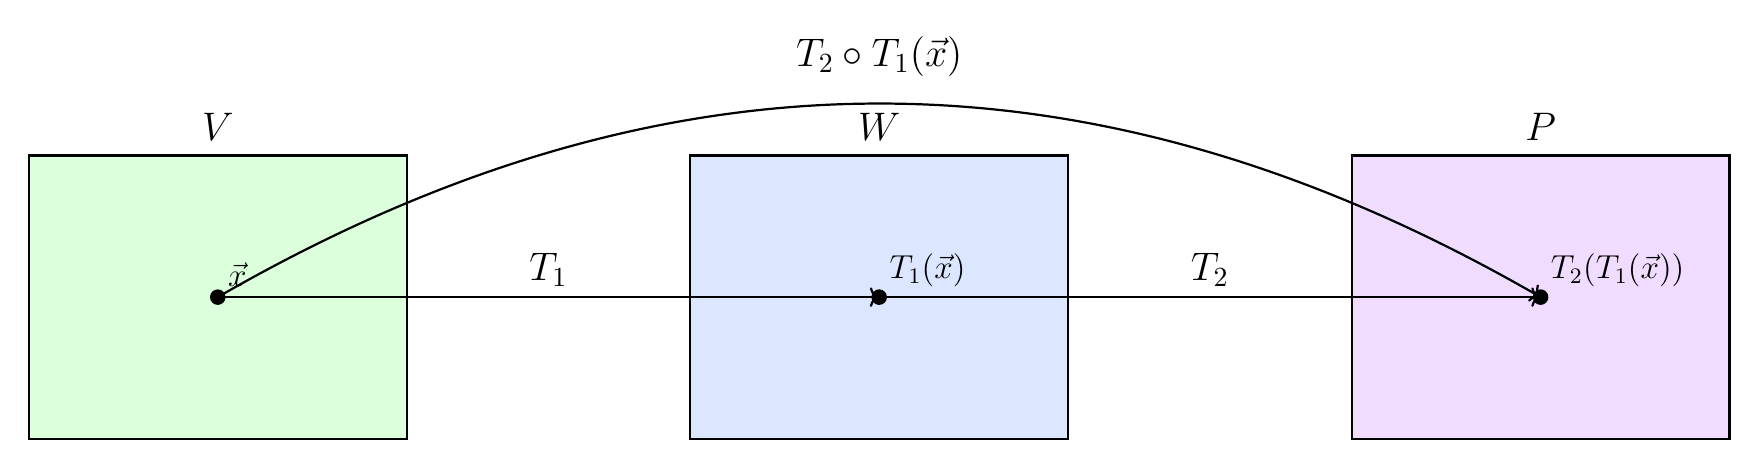
\begin{tikzpicture}[scale=1.2, thick]

  % Colors
  \definecolor{lightgreen}{RGB}{220,255,220}
  \definecolor{lightblue}{RGB}{220,230,255}
  \definecolor{lightpurple}{RGB}{240,220,255}

  % Plane V (domain)
  \filldraw[fill=lightgreen, draw=black] (-2,-1.5) rectangle (2,1.5);
  \node at (0,1.8) {\Large$V$};

  % Plane W (codomain)
  \filldraw[fill=lightblue, draw=black] (5,-1.5) rectangle (9,1.5);
  \node at (7,1.8) {\Large$W$};

  % Plane P (next space)
  \filldraw[fill=lightpurple, draw=black] (12,-1.5) rectangle (16,1.5);
  \node at (14,1.8) {\Large$P$};

  % Centered point x in V
  \filldraw[black] (0,0) circle (2pt) node[above right] {\large$\vec{x}$};

  % Centered point T(x) in W
  \filldraw[black] (7,0) circle (2pt) node[above right] {\large$T_1(\vec{x})$};

  % Arbitrary mapped point in P
  \filldraw[black] (14,0) circle (2pt) node[above right] {\large$T_2(T_1(\vec{x}))$};

  % Transformation Arrows
  \draw[->, thick] (0,0) -- (7,0) node[midway, above] {\Large$T_1$};
  \draw[->, thick] (7,0) -- (14,0) node[midway, above] {\Large$T_2$};

  % Curved composition arrow from V to P
  \draw[->, thick, bend left=30] (0,0) to node[midway, above, yshift=6pt] {\Large$T_2 \circ T_1(\vec{x})$} (14,0);

\end{tikzpicture}
\end{document}
